% ~ 6 pages
\chapter{Machine Learning}
\label{sec:ml}

Machine learning is the study of algorithms that are able to learn structure
from data (called training data) and can subsequently be used to make
predictions on unseen data. Examples for such algorithms are \emph{Boosted
  Decision Trees} (BDT) and \emph{Neural Networks} (NN) which are able to model
nonlinear problems without the need to supply an explicitly derived rule-set or
functional form. They often offer superior performance compared to linear models
or simple cut-based approaches at the cost of interpretability. Machine learning
techniques are widely used for the reconstruction of hadronic tau decays in the
ATLAS experiment. Aside from tau identification, they are used for track
classification, decay mode classification and energy calibration.

The focus lies on \todo{Worth a paragraph? Focus of what?} supervised learning,
which is concerned with learning models from labelled data (each example
consisting of explanatory variables and the dependent variable / label). This
domain includes regression for modelling a continous response and classification
for assigning class labels (e.g.\ signal or background) to an observation with
associated input variables.

This chapter gives an overview over the techniques used in this thesis starting
with a brief description of \emph{Boosted Decision Trees} that are used in
chapter~\ref{sec:bdt} for rejection of tau candidates originating from dijet
events. A comprehensive summary on \emph{Recurrent Neural Networks} is given
that are used for tau identification in chapter~\ref{sec:rnn} and additionally
for decay mode classification in chapter~\ref{sec:decaymode}. An overview of the
software frameworks used for this thesis concludes this chapter.

\section{Boosted Decision Trees}
\label{sec:bdt}

The following section describes a classification algorithm called \emph{Boosted
  Decision Trees}. It consists of an ensemble of decision trees that is created
by a meta-algorithm called \emph{boosting}. In
section~\ref{sec:ml_decision_trees} the decision tree algorithm is presented. A
brief overview of \emph{boosting} algorithms is given in
section~\ref{sec:ml_boosting}. The description focuses on binary classification
tasks aiming to discriminate between two distinct classes (hereafter called
signal and background).

\subsection{Decision Trees}
\label{sec:ml_decision_trees}

\begin{figure}[htb]
  \centering
  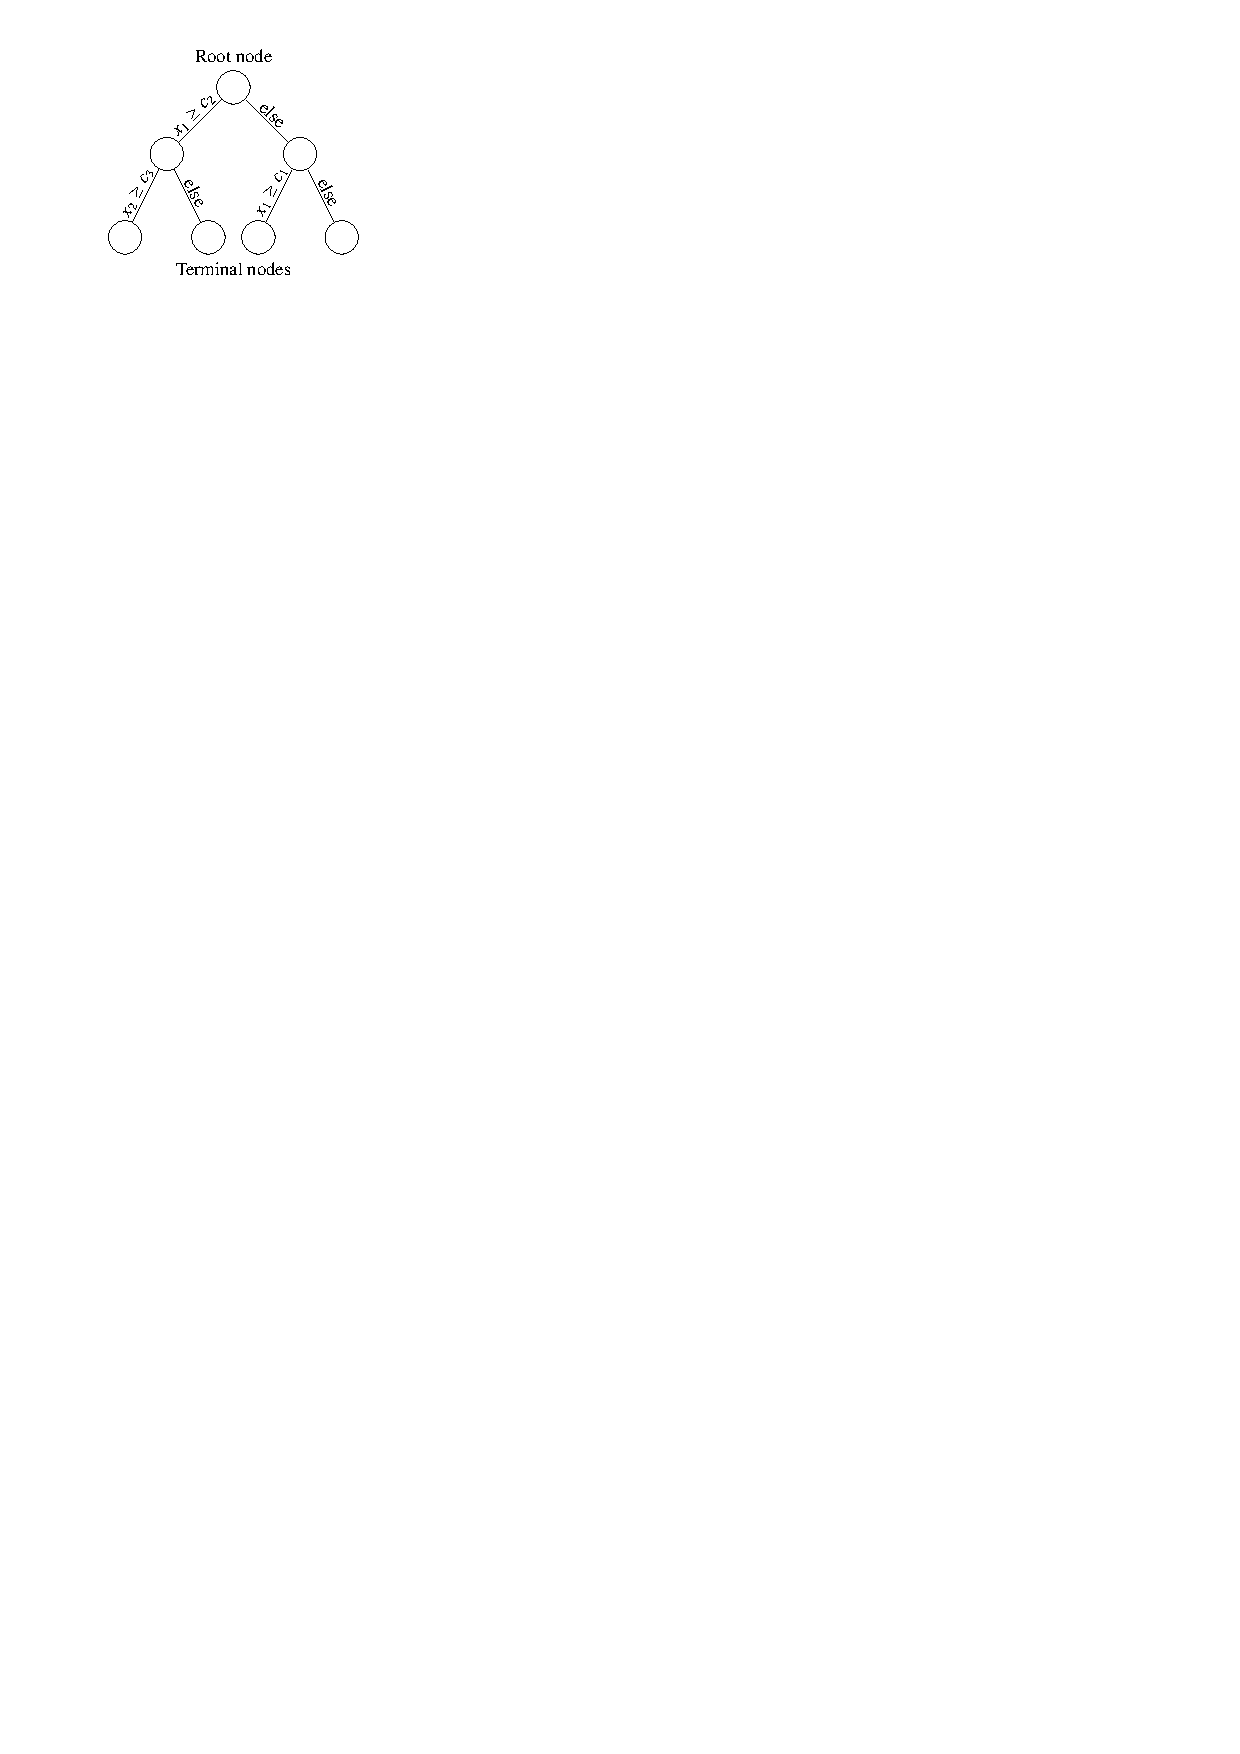
\includegraphics{./figures/theory/decision_tree.pdf}
  \caption{Binary tree structure of a decision tree with a depth~$d = 2$ and two
    input variables $x_1$, $x_2$. Adapted from \cite{esl}}
  \label{fig:decision_tree}
\end{figure}

\todo[inline]{Gini index: Probability to assign
  the correct label to a randomly picked observation when randomly
  assigning according to the distribution of labels in the sample
  (splits that split off pure background as well as signal are
  equivalent); Pruning?; Overfitting?}

A decision tree is a tree-based model that recursively partitions the space
spanned by the input variables into disjoint subregions by applying binary
splits on the coordinate axes until a stopping criterion is met. Frequently used
criteria include limiting the maximum depth of the tree or requiring a minimum
number of training examples in a node considered for further splitting.
Figure~\ref{fig:decision_tree} shows the binary tree structure of a decision
tree. The root node of the tree contains the full dataset which is subsequently
split into two nodes by a condition on a single input variable. The terminal
nodes (leaves) contain disjoint sub-samples of the full dataset with input
variables falling into distinct regions of the variable space. Each terminal
node is assigned the majority class of the subset of training data contained
within it. An alternative method to gauge the confidence of the decision is to
assign the signal purity.
% The subregions of the variable space defined by the terminal nodes Formally:
% majority class minimises classification error, signal purity minimises
% log-loss

A decision tree is grown using a greedy optimisation method, where each node is
split on the variable that gives the largest improvement according to a chosen
impurity measure. Commonly used for binary classification trees is the
\emph{Gini impurity} given by
\begin{align*}
  I_\text{G}(p) = 2 p_1 p_2 = 2 p (1 - p) \qquad \text{with} \qquad p \coloneqq p_1 = 1 - p_2 \eqcomma
\end{align*}
where $p_i$ is the purity of class~$i$ \cite{esl}. The best split is
chosen such that the mean of the Gini impurities of the resulting
nodes, weighted by the sum of event weights in each node, is
minimised.

\subsection{Boosting}
\label{sec:ml_boosting}

Boosting describes a family of machine learning meta-algorithms that are used to
build ensembles of base classifiers which aim to improve the overall predictive
power compared to a single model. The ensembles can be viewed as an additive
expansion of the underlying functional dependence in a set of basis functions
given by the base learner \cite{esl}. Boosting is commonly used in conjunction
with Decision Trees giving rise to so called \emph{Boosted Decision Trees}.

\todo{Hyperparameter number of trees}

\emph{AdaBoost} (Adaptive Boosting) is a boosting algorithm that forms a
weighted sum of the base classifier, where each classifier is trained on data
that is reweighted such that training examples that were previously incorrectly
classified contribute with higher weight than examples that were correctly
classified. \todo{\emph{AdaBoost} $\beta$ -- learning rate -- modifies boost
  weight} A generalisation of this method is called \emph{gradient boosting}
which allows the minimisation of an arbitrary differential loss function during
boosting. A loss function -- ya. Gradient boosting reproduces the
\emph{AdaBoost} algorithm if the exponential loss function $\exp(-f(x) y)$ is
used. In general for different loss functions no convenient methods of
minimising the loss exist and a gradient descent algorithm is used. A full
mathematical description of the algorithm is omitted for brevity and can be
found in \cite{friedman_gbm, esl}. Instead we focus on the major difference
between \emph{AdaBoost} and gradient boosting with binomial log-likelihood
$\log\left( 1 + \exp(-2 f(x) y) \right)$ (TMVA) loss. Regularisation using
shrinkage $\eta$.

\todo[inline]{TMVA: Real AdaBoost?; AdaBoost performance degrades in noisy
  settings due to exponential loss function \cite{esl} binomial log-likelihood
  more robust; AdaBoost performance degrades in noisy settings due to exp.\ loss
  function \cite{esl} -- binomial log-likelihood more robust}

\section{Artificial Neural Networks}
\label{sec:nn}

Artificial neural networks encompasses a large set of models that can be used as
approximations to a wide variety of non-linear functions \cite{hornik}. They can
be thought of as rules to compute a
mapping~\mbox{$\mathbb{R}^n \rightarrow \mathbb{R}^m$} between a set of
$n$~input variables and $m$~desired responses. The central idea is to repeatedly
compute intermediate representations of the inputs by applying transformations
and combining the final representation in a linear or logistic regression model.
Neural networks are typically organised into different \emph{layers} defining
the transformation that is applied on the layer inputs. Multiple layers
connected according to a computational graph form a network. This scheme allows
for great flexibility in building different models making neural networks highly
performing models in many areas of machine learning research \todo{Citation}.

The following sections introduce concepts needed to understand the models used
for various (sequence) classification tasks given in this thesis. Matrices and
vectors are denoted using bold symbols e.g.\ input variables~$\mathbf{x}$ and
responses~$\mathbf{y}$ of a layer or network.

\subsection{Feedforward Neural Networks}
\label{sec:nn_feedforward}
Feedforward neural networks are networks in which information flows strictly in
the forward direction, disallowing feedback loops (e.g.\ recurrent connections
introduced in section~\ref{sec:rnn_theory}) between input and output of a single
layer. An example of a simple feedforward neural networks is the multi-layer
perceptron consisting of a number of input neurons $\mathbf{x}$ used to pass the
discriminating variables to the network, an output layer with activation
$\mathbf{y}$ and several intermediate (hidden) layers connecting input and
output layer.
\begin{figure}[htb]
  \centering
  \begin{minipage}[t]{0.55\textwidth}
    \centering
    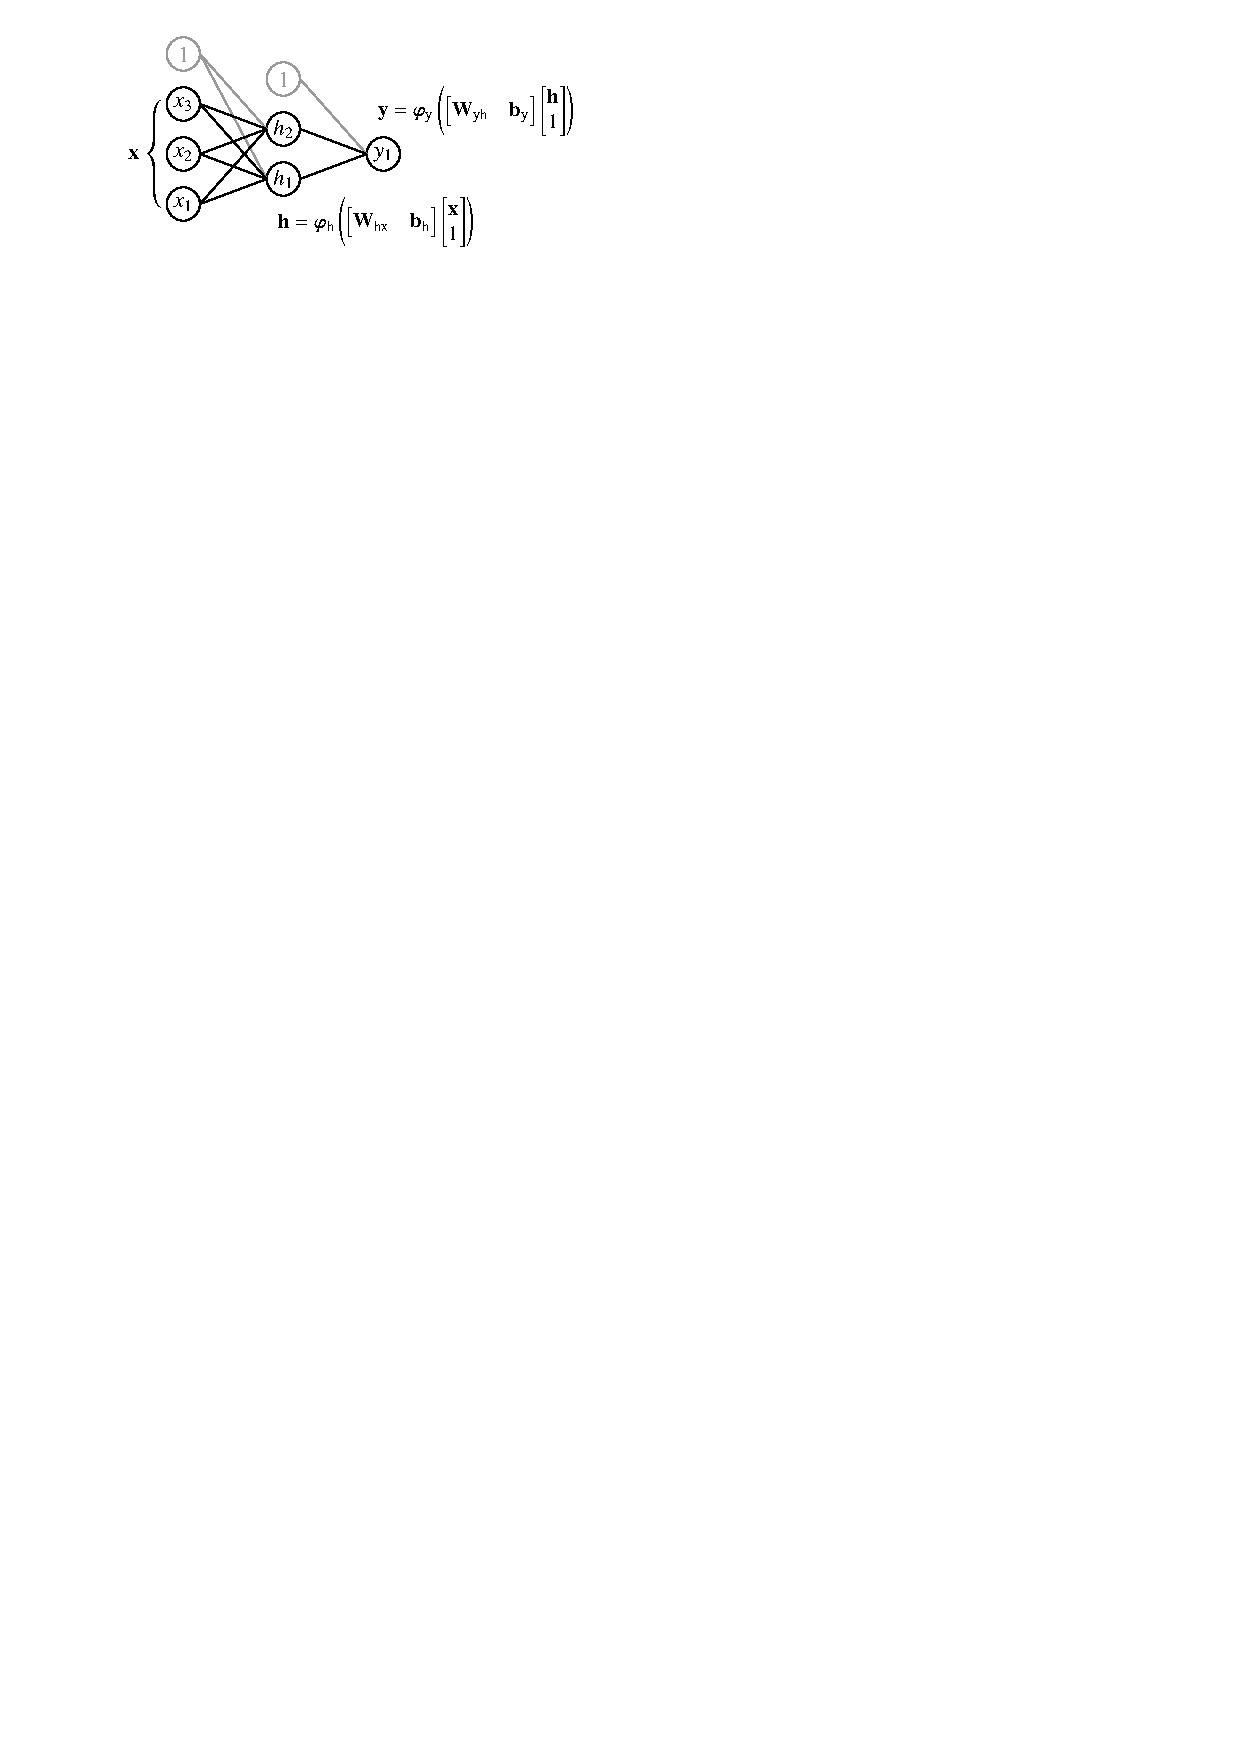
\includegraphics{./figures/theory/mlp.pdf}
    \captionof{figure}{Multi-layer perceptron with input neurons $\mathbf{x}$,
      hidden layer activation $\mathbf{h}$ and output activation $\mathbf{y}$.
      The layers are connected via weights $\mathbf{W}$ and optional biases
      $\mathbf{b}$. Activations are given after applying an element-wise
      activation function $\bm{\varphi}$.}
    \label{fig:multi_layer_perceptron}
  \end{minipage}\hfill
  \begin{minipage}[t]{0.4\textwidth}
    \centering
    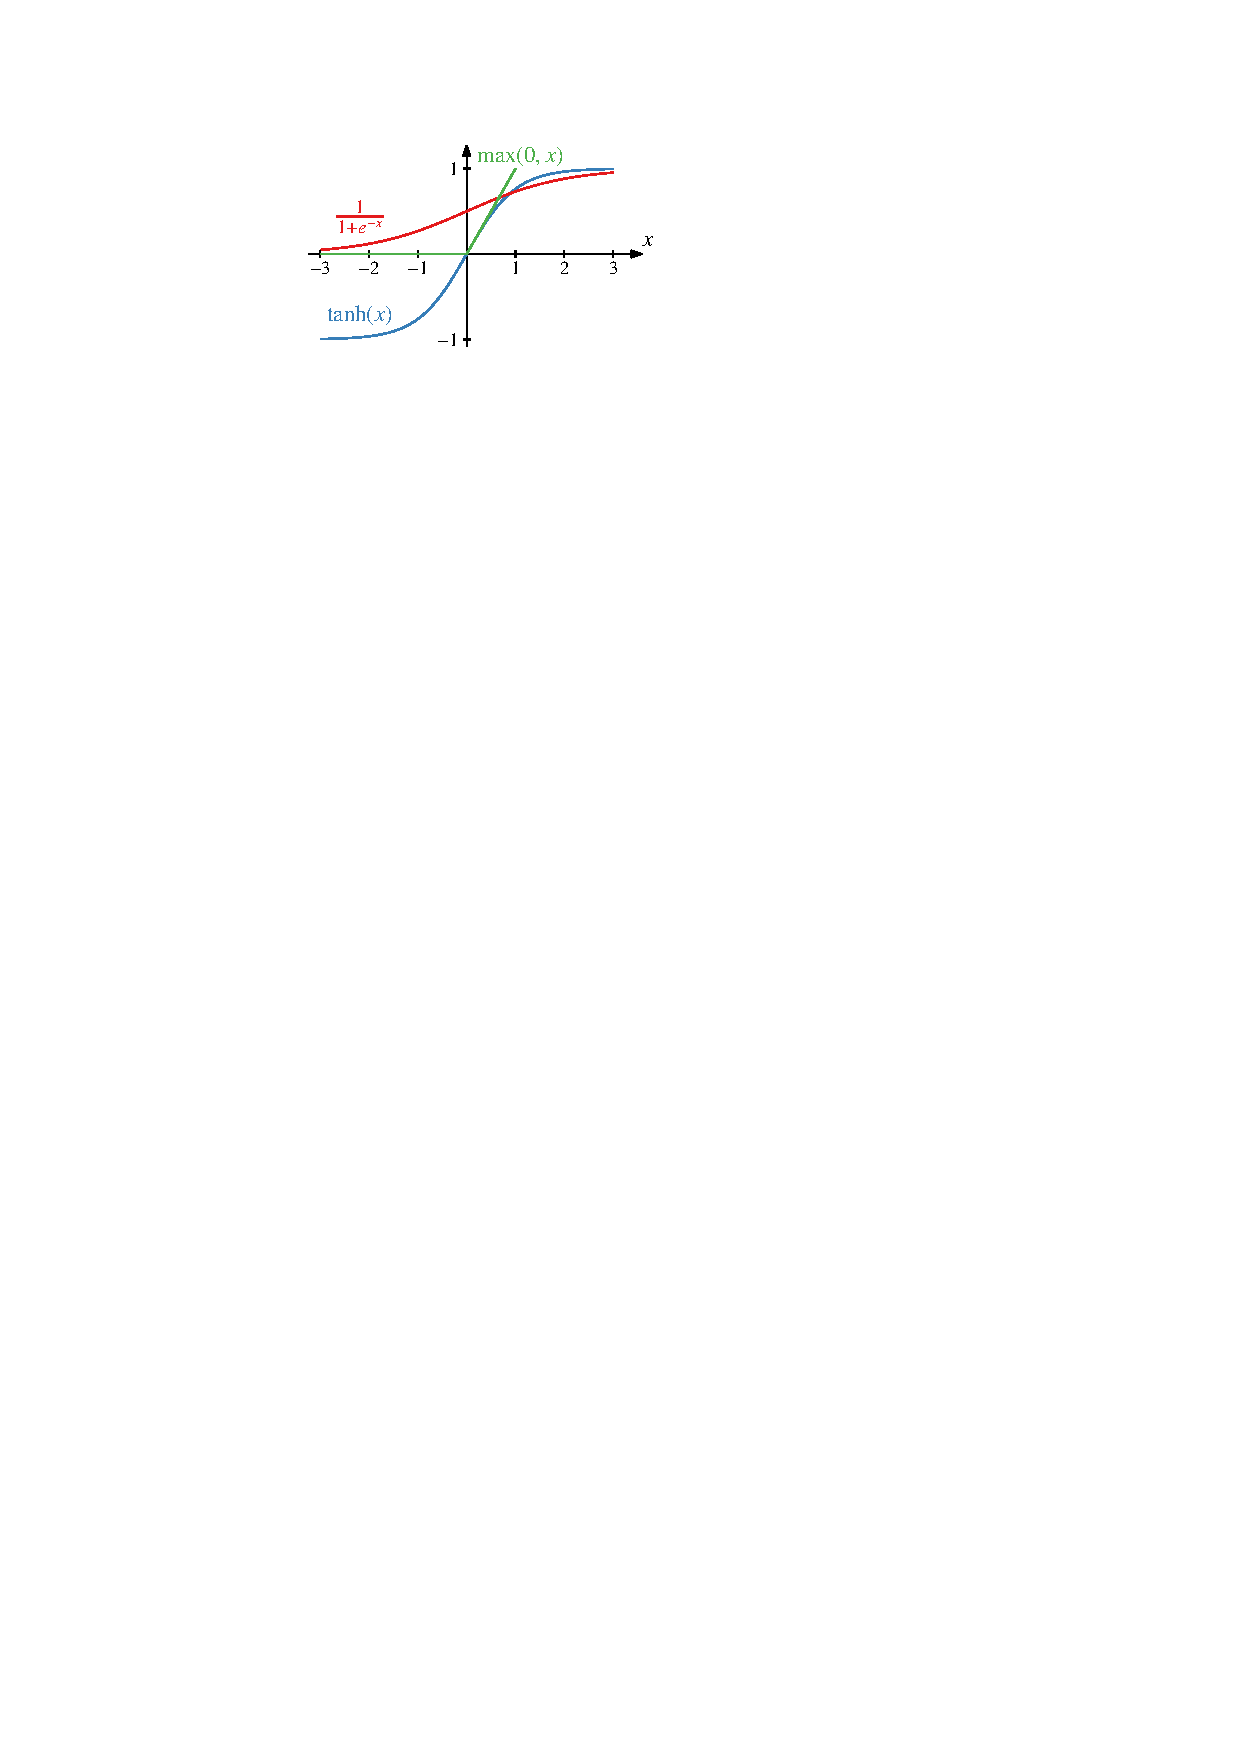
\includegraphics{./figures/theory/activation_functions.pdf}
    \captionof{figure}{Commonly used activation functions: logistic function (red),
      hyperbolic tangent (blue), and rectified linear units (green).}
    \label{fig:activation_functions}
  \end{minipage}
\end{figure}
In figure~\ref{fig:multi_layer_perceptron} a multi-layer perceptron with a
single hidden layer is shown. Two layers are connected by an affine
transformation and subsequent application of an element-wise, non-linear and
differentiable activation function~$\bm{\varphi}$. These layers are called dense
or densely-connected layers, as each neuron is connected to every other neuron
in the neighboring layer. For the case depicted in
figure~\ref{fig:multi_layer_perceptron} the activations in the hidden
layer~$\mathbf{h}$ and the output layer~$\mathbf{y}$ are given by:
\begin{align*}
  &\mathbf{h} = \bm{\varphi}_{\text{h}}(\mathbf{W}_{\text{hx}} \mathbf{x} + \mathbf{b}_{\text{h}})
  &\mathbf{y} = \bm{\varphi}_{\text{y}}(\mathbf{W}_{\text{yh}} \mathbf{h} + \mathbf{b}_{\text{y}}) \eqcomma
\end{align*}
where $\mathbf{W}$ are weight matrices determining the weight of each connection
between two neurons and $\mathbf{b}$ are optional bias vectors. Generally the
sizes of the hidden layers as well as the choice of the activation functions are
hyperparameters of the model. The size of the input and output layer is given by
the number of input variables and the number of desired outputs respectively.
Moreover the activation function of the output layer is constrained by the
underlying task. For binary classification the logistic
function~\smash{$\sigma(x) = (1 + \exp(-x))^{-1}$} is applied to a single output
neuron giving the probability of an observation being of the positive class
(e.g.\ signal). For multi-class classification the number of outputs neurons is
chosen to be equal to the number of classes that need to be distinguished and
the \emph{softmax} function \cite{esl, bishop}
\begin{align*}
  \varphi_i(\mathbf{x}) = \frac{e^{x_i}}{\sum_j e^{x_j}}
\end{align*}
is chosen as the activation function, where~$\varphi_i(\mathbf{x})$ is the
activation of the $i$-th neuron and $x_i$ the value of the neuron before
activation. The \emph{softmax} function ensures that the sum of all activations
in a layer equals to one, such that they can be interpreted as class
probabilities. Activation functions that are commonly used for the intermediate
layers are depicted in figure~\ref{fig:activation_functions}.

So far the networks were viewed as non-linear parametric functions mapping input
variables~$\mathbf{x}$ to a response~$\mathbf{y}$ without regarding the choice
of parameters (i.e.\ weights and biases of each layer). The model parameters are
determined using gradient descent by minimising an objective function (training
of the model). The objective function penalises errors in the model's
predictions and is commonly called the loss function. Categorical cross-entropy
is generally used for $K$-class classification tasks. For an observation
belonging to a class~$k \in \{1, \dots, K\}$ it is defined as \cite{esl, bishop}
\begin{align*}
  L\left(k, \mathbf{p}(\mathbf{x}) \right) = - \log\left( p_k(\mathbf{x}) \right) \eqcomma
\end{align*}
where~$\mathbf{p}(\mathbf{x}) = \mathbf{y}(\mathbf{x})$ is the probabilistic interpretation
of the model with class probabilities~$p_k$ (after \emph{softmax} activation)
and discriminating variables~$\mathbf{x}$. For binary
classification it is sufficient to give the predicted probability~$p$ (after
logistic sigmoid activation) for the positive class such that the binary
cross-entropy can be written as
\begin{align*}
  L(t, p(\mathbf{x})) = -t \, \log(p(\mathbf{x})) - (1 - t) \, \log(1 - p(\mathbf{x})) \eqcomma
\end{align*}
with the binary indicator~$t$ encoding the true class (0 for the negative and 1
for the positive class). When looking at a subset of observations with event
weights~$w_i$ the loss~$\mathcal{L}$ is defined as \todo{Somehow denote subset
  of data}
\begin{align*}
  &\mathcal{L} = \frac{\sum_i w_i L_i}{\sum_j w_j}
    \qquad \text{with} \qquad
    L_i = L\left(k_i, \mathbf{p}(\mathbf{x}_i)\right) \eqcomma
\end{align*}
which in case of the cross-entropy can be interpreted as the negative
log-likelihood of the (generalised) \textsc{Bernoulli} distribution with respect
to the model parameters given the observed subset of data \cite{bishop}.

The task of finding the parameters of the model minimising the expected loss
(maximising the likelihood) on a set of training data is solved using stochastic
gradient descent. This requires information on the gradient of the
loss~$\mathcal{L}(\mathbf{w})$ with respect to the model weights~$\mathbf{w}$
(biases can be absorbed into the weight matrices as shown in
figure~\ref{fig:multi_layer_perceptron}). Each layer in the computational graph
making up the network has a well-defined derivative such that by repeatedly
applying the chain rule for partial derivatives the gradient
$\nabla_\mathbf{w} \mathcal{L}(\mathbf{w})$ can be calculated symbolically. This
procedure is generally known as error backpropagation or \emph{BackProp}
\cite{bishop, lecun-backprop}. Knowing the gradient of the loss an iterative
optimisation method called mini-batch (stochastic\footnote{The gradient of the
  loss on the full training sample is approximated by the gradient on a
  mini-batch.}) gradient descent is employed. Initially the weights are
randomised to small values and biases set to zero. The set of training examples
is divided into subsets of fixed size called mini-batches. In an iterative
procedure the weights are updated according to
\begin{align*}
  \mathbf{w}_{t+1} = \mathbf{w}_t - \eta \, \nabla_\mathbf{w} \mathcal{L}(\mathbf{w}_t) \eqcomma
\end{align*}
where $\eta > 0$ is called the learning rate and
$\nabla_\mathbf{w} \mathcal{L}(\mathbf{w}_t)$ is the gradient evaluated on the
mini-batch. One pass over all mini-batches is called an epoch and typically
multiple epochs are required to train a model. In practice the loss on an
independent validation set is observed and the procedure is stopped when the
validation loss stops decreasing.

\todo[inline]{Find more references; Large penalties to predictions that are far
  off; Perfect classifiers have loss of zero (can always be reached with complex
  models); Cross validation?}

\subsection{Recurrent Neural Networks}
\label{sec:rnn_theory}
Events reconstructed in particle detectors contain multiple reconstructed
objects of the same type e.g.\ particle tracks or clusters in the calorimeter.
The rigid structure of feedforward neural networks does not offer a general
method to classify events with variable numbers of objects. Recurrent neural
networks~(RNN) provide an approach to sequence classification by introducing
cyclical connections within layers, i.e.\ units being connected to themselves.
These recurrent connections allow decisions to be made in the context of the
sequence (e.g.\ obeying constraints due to momentum conservation) by making the
network able to store information on previous objects \cite{graves}.

The \textsc{Elman} network is introduced and will be extended to the long
short-term memory~(LSTM) architecture used in this thesis. Biases are omitted in
the following description as they can be absorbed into the weight matrices.

\subsubsection{Simple Recurrent Networks}
\label{sec:simple_recurrent_networks}
Recurrent neural networks are able to map a sequence of input variables to a
sequence of outputs. Both sequences can have arbitrary lengths between different
observations. An example of a \emph{Simple Recurrent Network} is the
\textsc{Elman} network depicted in figure~\ref{fig:schematic_elman_rnn}. It is
shown in a compact notation as well as unfolded in time\footnote{Nomenclature
  originates from RNNs being used to predict time series.} representing it as a
feedforward network with weights shared between time steps.
\begin{figure}[htb]
  \centering
  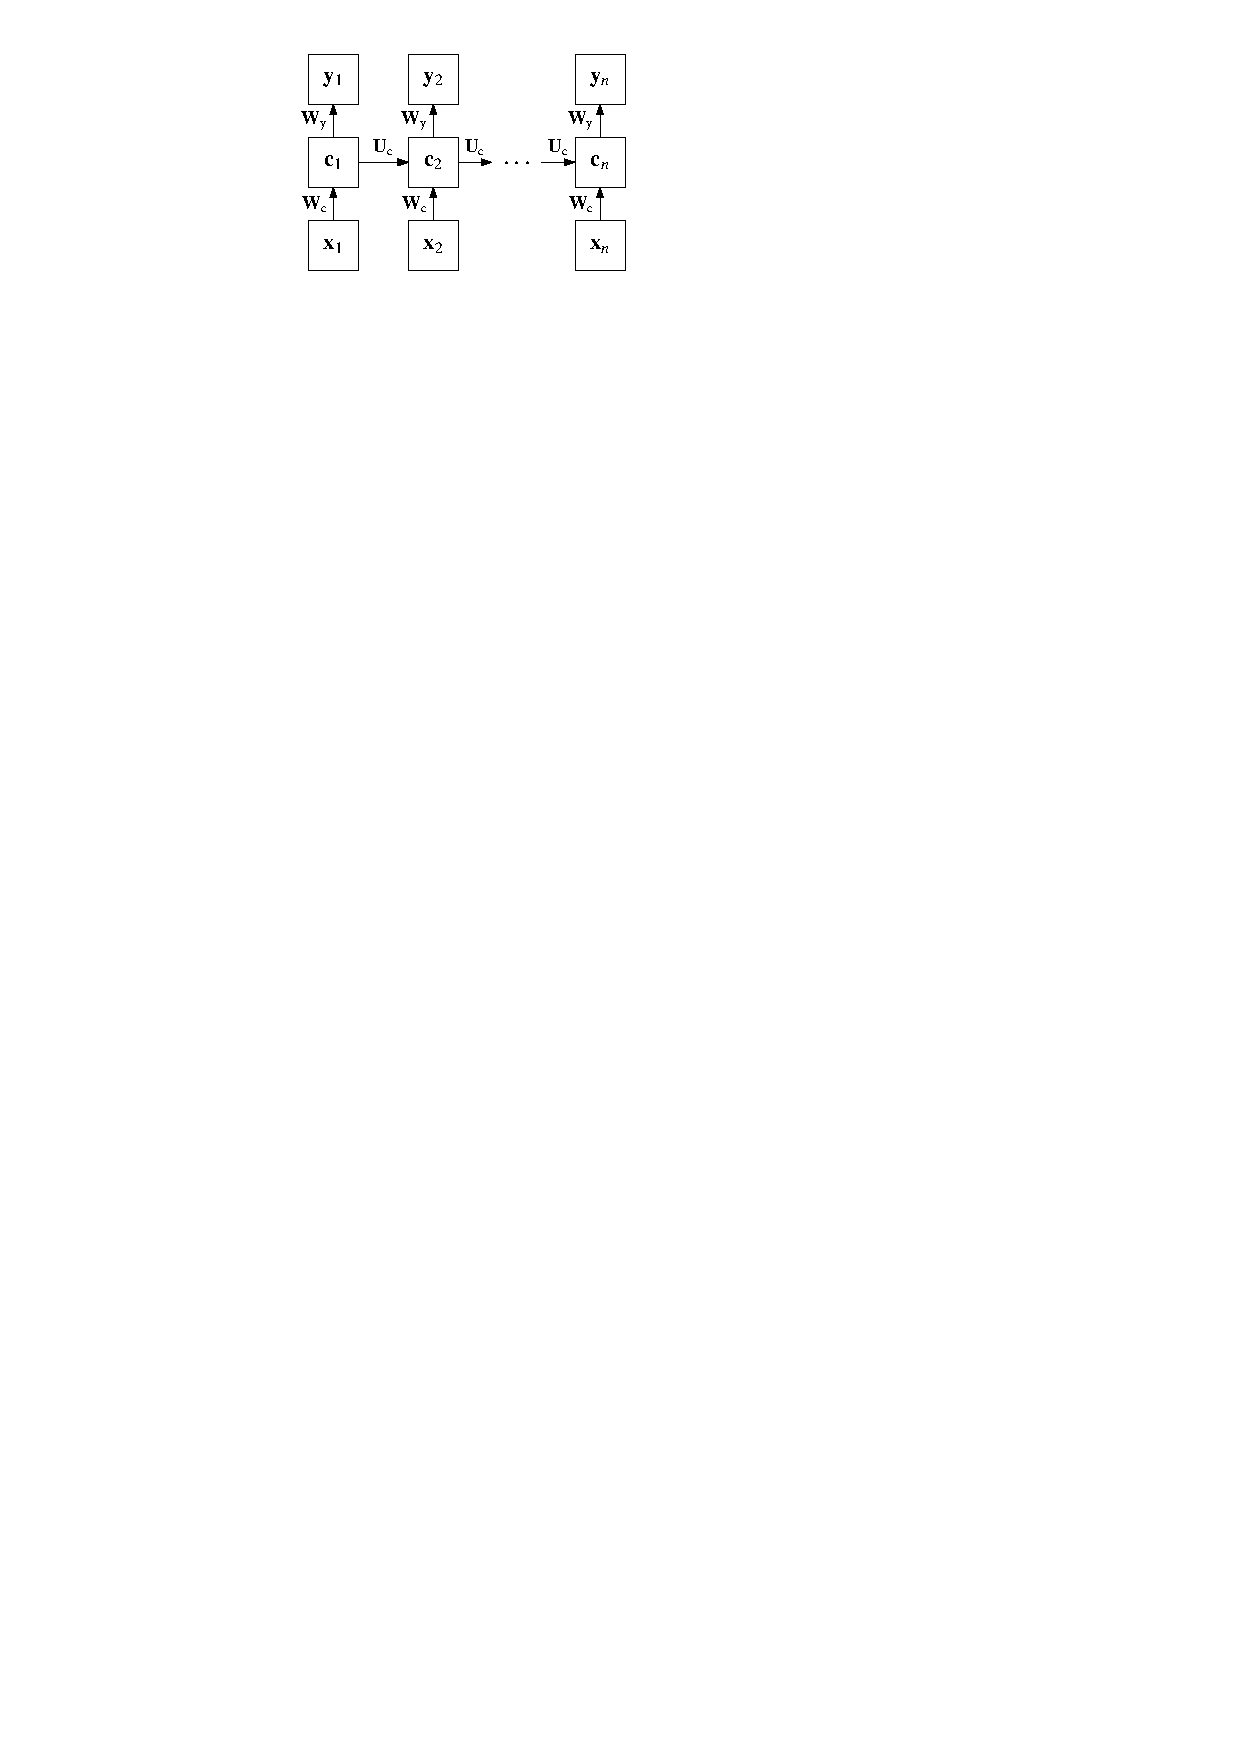
\includegraphics{./figures/theory/elman_rnn.pdf}
  \caption{Schematic depiction of an \textsc{Elman} network in compact form with
    a recurrent connection and after unfolding the network in time. The black
    square at the recurrent connection represents a delay of one time step.
    Application of nonlinear activation functions are omitted. The figure is
    adapted from \cite{lecun_bengio_hinton_DL}.}
  \label{fig:schematic_elman_rnn}
\end{figure}
The input sequence~$\left( \mathbf{x}_i \right)_{i=1}^n$ is processed one
element at a time. The sequence of cell states~$\mathbf{c}_t$ and
outputs~$\mathbf{y}_t$ can be computed by iteratively applying the rule
\begin{align*}
  \mathbf{c}_t &= \bm{\varphi}_{\text{c}}\Big( \mathbf{W}_{\text{c}} \mathbf{x}_{t} + \mathbf{U}_{\text{c}} \mathbf{y}_{t-1} \Big)
  &\mathbf{y}_t &= \bm{\varphi}_{\text{y}}\Big( \mathbf{W}_{\text{y}} \mathbf{c}_{t} \Big)
\end{align*}
with weights~$\mathbf{W}$, recurrent weights~$\mathbf{U}$ and activation
functions~$\bm{\varphi}$, while incrementing the time step $t$ \cite{elman,
  graves}. The initial cell state is often set to $\mathbf{c}_0 = \mathbf{0}$
but the particular choice can differ between implementations. All weights are
shared between time steps which allows sequences of arbitrary length to be
processed by the network. The cell state~$\mathbf{c}_t$ at each time step~$t$ is
updated using the external input~$\mathbf{x}_t$ as well as the cell
state~$\mathbf{c}_{t-1}$ of the previous time step ($\mathbf{c}_0 = \mathbf{0}$)
forming the recurrent connection. This allows the a memory of previous inputs to
persist in the internal state of the network thus enabling the
output~$\mathbf{y}_t$, which is calculated from the cell state, to depend on the
history of the sequence. As simple recurrent neural networks process the input
sequence in a predefined direction, only the past information can influence the
output at a specific time step making the order of the input sequence important.
An architecture allowing the context (past and future) to influence the output
at a given time~$t$ are bidirectional RNNs but will not further discussed. The
evaluation of the gradient for the training process follows the same principles
used for feedforward neural networks but now also considering that the chain
rule has to be applied for each time step and one has to consider that the
weights between time steps are shared (\emph{backpropagation through time}
\cite{williams_zipser}). After unfolding the network in time the training is
analogous to that of deep feedforward neural networks.

In this thesis RNNs are used for the classification of a sequence of
reconstructed objects in its entirety (as opposed to classifying each element in
the sequence). For this task the full output sequence of the recurrent network
is not needed, such that only the output of the last time step is used. Simple
Recurrent Networks like the \textsc{Elman} network show that the gradient signal
decays with each time step such that it is difficult to learn long-term
dependencies in the input sequence \cite{hochreiter, lecun_bengio_hinton_DL}
\todo{This is due to the repeated application of the activation function e.g.\
  $\tanh$ in the recurrent connection leading to a exponential decay of the
  gradient -- also affects feedforward networks}. The following section will
present an extension to this architecture enabling the network to learn
long-term dependencies.

\subsubsection{Long Short-Term Memory}
\label{sec:lstm}
The long short-term memory (LSTM) network developed in~\cite{lstm} solves the
\emph{vanishing gradient problem} that affects simple recurrent networks by
introducing multiplicative gates that control the flow of information in the
network. In figure~\ref{fig:schematic_lstm} a schematic depiction of an unfolded
LSTM at time~$t$ is shown.
\begin{figure}[htb]
  \centering
  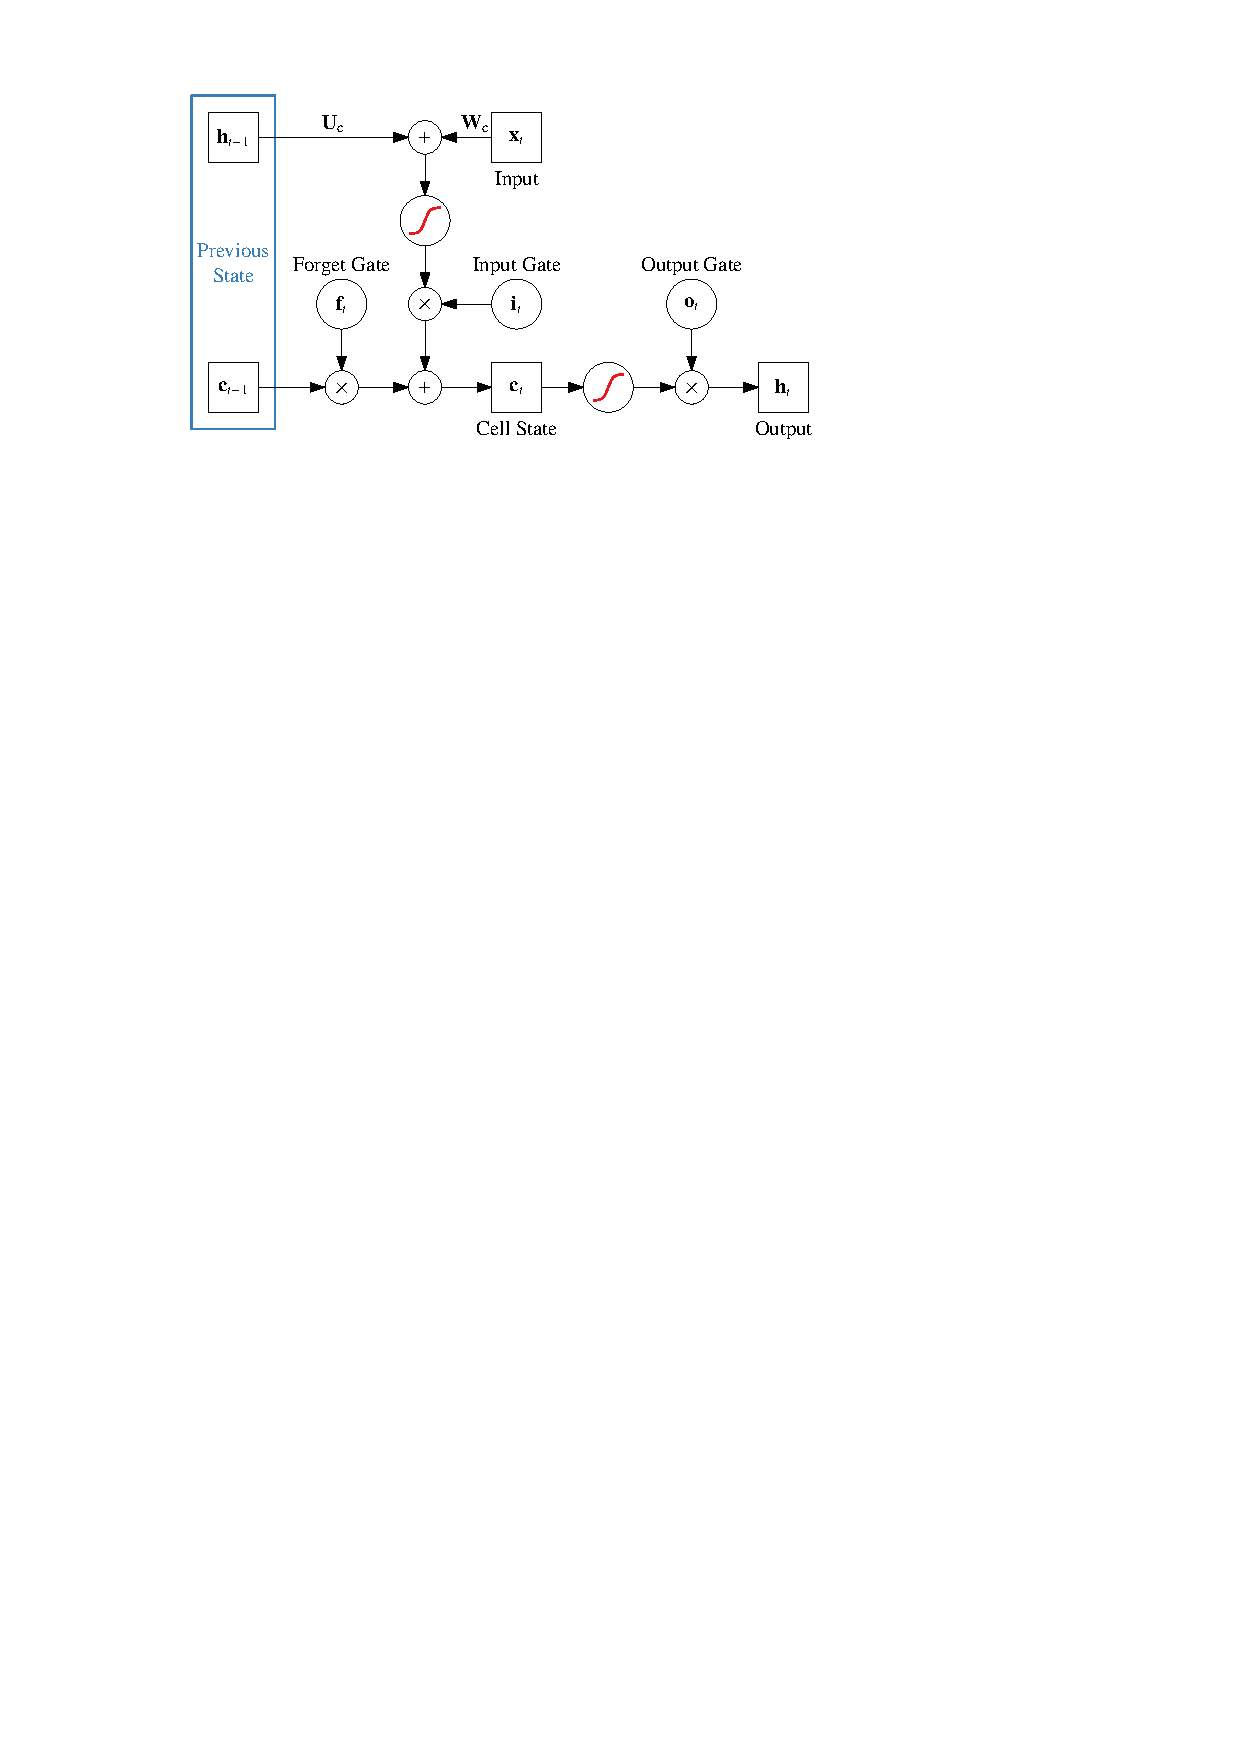
\includegraphics{./figures/theory/LSTM.pdf}
  \caption{Schematic description of a LSTM-cell.}
  \label{fig:schematic_lstm}
\end{figure}
The LSTM represents a (differentiable) memory cell with three gates called the
input, output and forget gate. The gate vectors are given by
\begin{align*}
  \mathbf{f}_{t} &= \bm{\varphi}_{\text{g}}\left( \mathbf{W}_{\text{f}} \mathbf{x}_{t} + \mathbf{U}_{\text{f}} \mathbf{y}_{t-1} \right) &
  \mathbf{i}_{t} &= \bm{\varphi}_{\text{g}}\left( \mathbf{W}_{\text{i}} \mathbf{x}_{t} + \mathbf{U}_{\text{i}} \mathbf{y}_{t-1} \right) &
  \mathbf{o}_{t} &= \bm{\varphi}_{\text{g}}\left( \mathbf{W}_{\text{o}} \mathbf{x}_{t} + \mathbf{U}_{\text{o}} \mathbf{y}_{t-1} \right)
\end{align*}
with separate weights~$W$ and recurrent weights~$U$ for each gate
($\mathbf{y_0} = \mathbf{0}$). The gate activation
function~$\bm{\varphi}_\text{g}$ is typically the logistic function as it maps
real values into the interval $[0, 1]$. Notably the gate activations depend on
the input~$\mathbf{x}_t$ at time~$t$ as well as the output~$\mathbf{y}_{t-1}$ of
the LSTM at the previous time step\todo{such that memory access patterns depend
  on the inputs and history}. To understand how the gating controls the flow of
information in a LSTM one looks at the update of the cell state $\mathbf{c}$
with each time step:
\begin{align*}
  \mathbf{c}_{t} &= \mathbf{f}_{t} \circ \mathbf{c}_{t-1}
                   + \mathbf{i}_{t} \circ \bm{\varphi}_{\text{c}}(
                   \mathbf{W}_{\text{c}} \mathbf{x}_{t}+ \mathbf{U}_{\text{c}}
                   \mathbf{y}_{t-1} ) \eqcomma
\end{align*}
where $\circ$ denotes the element-wise multiplication of two column vectors
\todo{whats $\bm{\varphi}$} and $\mathbf{c}_0 = \mathbf{0}$. The input gate
controls how much information from the input~$\mathbf{x}_t$ and
output~$\mathbf{y}_{t-1}$ is taken into the cell state therefore avoiding the
inclusion of irrelevant information into the cell state. A main feature of the
LSTM architecture is the direct connection of cell states between two successive
time steps via the forget gate solving the \emph{vanishing gradient problem}.
The forget gate enables the network to gradually reset its internal state once
stored information has become irrelevant. Finally the output~$\mathbf{y}_t$ is
calculated using using
\begin{align*}
  \mathbf{y}_{t} &= \mathbf{o}_{t} \circ \bm{\varphi}_{\text{y}}(\mathbf{c}_{t}) \eqcomma
\end{align*}
where~$\bm{\varphi}_y$ is usually the hyperbolic tangent. The activation of the
output gate determines how much of the cell state is presented at the output of
the network. Overall the multiplicative gating of the LSTM allows information to
persist in its internal state over a long period of time with gates resembling
the write, read and reset gates of conventional memory cells.

Variables:
\begin{itemize}
\item $x_t$: input vector
\item $h_t$: output vector
\item $c_t$: cell state vector
\item $W$, $U$ and $b$: (recurrent -- $U$) weight matrices and bias vector
\item $f_t$, $i_t$ and $o_t$: gate vectors
  \begin{itemize}
  \item $f_t$: forget gate vector
  \item $i_t$: input gate vector
  \item $o_t$: output gate vector
  \end{itemize}
\end{itemize}

Activation functions:
\begin{itemize}
\item $\sigma_g$: element-wise sigmoid function (Gate activation -- recurrent
  activation)
\item $\sigma_c$: element-wise hyperbolic tangent (Cell activation -- recurrent
  activation)
\item $\sigma_h$: element-wise hyperbolic tangent (Output activation)
\end{itemize}

Gated Recurrent Unit (GRU) as an alternative.

Bidirectional Recurrent Neural Networks: consider past and future context when
classifying. Present the training sequence forwards and backwards to two
separate recurrent neural networks connected to the same output layer.

\section{Technical Setup}
\label{sec:tech_setup}

TMVA

Frameworks used for this thesis (theano \cite{theano}, keras \cite{keras})
SciPy \cite{scipy}
Numpy \cite{numpy}
h5py

Optimiser: Adam

Masking layer

Biases are always used.

%%% Local Variables:
%%% mode: latex
%%% TeX-master: "mythesis"
%%% End:
